\section{Results}\label{sec:results}

This section evaluates all strategies out-of-sample on the test period (January 2011 to November 2025, 167 months). Each method produces a long-only, value-weighted, top-decile portfolio rebalanced monthly with one-way transaction costs of 10 basis points. Portfolio construction details and performance metric definitions are provided in Appendix~\ref{app:portfolio}. Feature importance is assessed via SHAP values \citep{Lundberg2017} for XGBoost and coefficient analysis for logistic regression; the methodological details are in Appendix~\ref{app:feature_importance}.

The analysis proceeds in five stages. First, Section~\ref{sec:performance_results} compares the overall performance of the ten strategies. Section~\ref{sec:regime_results} decomposes performance by market regime, revealing that the main benefit of the regime-conditioned models lies in calm-period stock selection rather than crash avoidance. Section~\ref{sec:decomposition} isolates the contributions of lookback flexibility, fundamental characteristics, and the regime signal $\pi_t^{\text{filter}}$ to the observed Sharpe ratio improvement. Section~\ref{sec:feature_results} examines which features drive the predictions through coefficient analysis and SHAP values. Finally, Section~\ref{sec:context_results} synthesises these findings into the central insight of the thesis: that $\pi_t^{\text{filter}}$ functions as a context variable that reveals the regime-dependent structure of cross-sectional momentum.

\subsection{Portfolio Performance}\label{sec:performance_results}

Table~\ref{tab:performance} reports out-of-sample performance for all strategies. The regime-conditioned methods (M1 and M2) substantially outperform both the market benchmark and the unconditional momentum baselines.

\begin{table}[htbp]
\centering
\caption{Out-of-sample portfolio performance.}
\label{tab:performance}
\small
\begin{tabular}{l r r r r r r r}
\toprule
 & Ann.\ Ret & Ann.\ Vol & Sharpe & 95\% CI & Max DD & NW $t$ & Final \$ \\
\midrule
Market & 11.9% & 14.6% & 0.84 & [0.40,\,1.44] & -24.7% & -- & 4.8 \\
\midrule
Fixed 12-mo mom & -1.9% & 26.1% & 0.06 & [-0.48,\,0.51] & -72.3% & -1.22 & 0.8 \\
Fixed 1-mo mom & 3.1% & 17.6% & 0.26 & [-0.24,\,0.67] & -30.2% & -1.35 & 1.5 \\
M0: Formula & 2.4% & 23.4% & 0.22 & [-0.28,\,0.61] & -56.9% & -0.94 & 1.4 \\
M1: LR (mom+$\pi$) & -1.6% & 15.1% & -0.03 & [-0.38,\,0.45] & -43.1% & -2.48** & 0.8 \\
M1: LR & -0.6% & 15.7% & 0.04 & [-0.52,\,0.62] & -54.4% & -1.79* & 0.9 \\
M2: XGB (mom+$\pi$) & 9.4% & 20.3% & 0.54 & [0.14,\,0.96] & -30.6% & -0.26 & 3.5 \\
M2: XGB & 10.3% & 15.1% & 0.73 & [0.41,\,1.10] & -17.1% & -0.32 & 3.9 \\
\midrule
GHM SLOW & -1.8% & 26.1% & 0.07 & [-0.46,\,0.51] & -72.3% & -1.22 & 0.8 \\
GHM MED & 0.2% & 21.7% & 0.12 & [-0.39,\,0.55] & -62.5% & -1.40 & 1.0 \\
GHM FAST & 3.1% & 17.6% & 0.26 & [-0.24,\,0.69] & -30.3% & -1.35 & 1.5 \\
GHM DYN & -2.1% & 22.8% & 0.03 & [-0.47,\,0.51] & -69.5% & -1.54 & 0.7 \\
\bottomrule
\end{tabular}

\medskip
\small
\textbf{Notes:} This table reports annualized return, annualized volatility, Sharpe ratio, 95\% block bootstrap confidence interval on the Sharpe ratio (block length = 12 months, 10{,}000 replications), maximum drawdown, Newey--West $t$-statistic for mean excess return over the market (HAC standard errors, 6 lags), and terminal wealth from \$1 invested. All strategies are long-short (top-decile long, bottom-decile short), value-weighted using NYSE breakpoints, and net of 10\,bps one-way transaction costs applied to both legs. The test period is January 2011 to November 2025 (167 months). ``mom+$\pi$'' denotes models trained on the 12 momentum lookbacks and the regime signal only, excluding fundamental features. $^{*}$\,$p<0.10$; $^{**}$\,$p<0.05$; $^{***}$\,$p<0.01$.
\end{table}

The logistic regression (M1) achieves a Sharpe ratio of 1.03 with the lowest annualised volatility among all active strategies (14.5\%), matching the market's volatility while delivering 14.8\% annualised returns versus 11.9\% for the market. Its maximum drawdown of $-$25.2\% is comparable to the market's $-$24.7\%, indicating effective downside protection. Importantly, M1's Sharpe ratio is statistically significant: the Newey--West $t$-statistic for its excess return over the market is 2.92 ($p < 0.01$), and the block bootstrap 95\% confidence interval on its Sharpe ratio ($[0.55, 1.61]$) excludes zero.

The XGBoost regressor (M2) generates the highest raw returns at 21.6\% annualised, with a Sharpe ratio of 1.01. Relative to M1, it trades higher returns for higher volatility (21.8\%), but its maximum drawdown of $-$26.1\% remains well below the fixed momentum and M0 strategies (which suffer drawdowns of $-$29.7\% to $-$36.5\%). M2's Newey--West $t$-statistic is 2.78 ($p < 0.01$), confirming that its outperformance is not a statistical artefact.

The deterministic formula (M0), which uses $\pi_t^{\text{filter}}$ only to select a momentum lookback horizon, achieves a Sharpe of 0.73. While this modestly exceeds fixed 12-month momentum (0.70), it falls well short of the machine learning methods. The formula cannot capture the nonlinear interactions between the regime signal and the full feature set that M1 and M2 exploit.

\begin{figure}[htbp]
    \centering
    
\includegraphics[width=\textwidth]{cs_performance.png}
    \caption{Cumulative wealth paths for all strategies (log scale), starting from \$1 in January 2011. M2 (XGBoost) achieves the highest terminal wealth (\$14.70), followed by M1 (logistic regression, \$6.80). Both regime-conditioned methods substantially outperform the market and unconditional momentum benchmarks.}
    \label{fig:cumulative}
\end{figure}

The GHM benchmark strategies, which use backward-looking market return momentum to classify regimes, achieve Sharpe ratios between 0.70 and 0.80. The best GHM variant (DYN, Sharpe 0.80) is outperformed by both M1 and M2, suggesting that real-time stress indicators (volatility, return dispersion, drawdown, market participation) provide a richer regime signal than trailing market returns alone.

\begin{figure}[htbp]
    \centering
    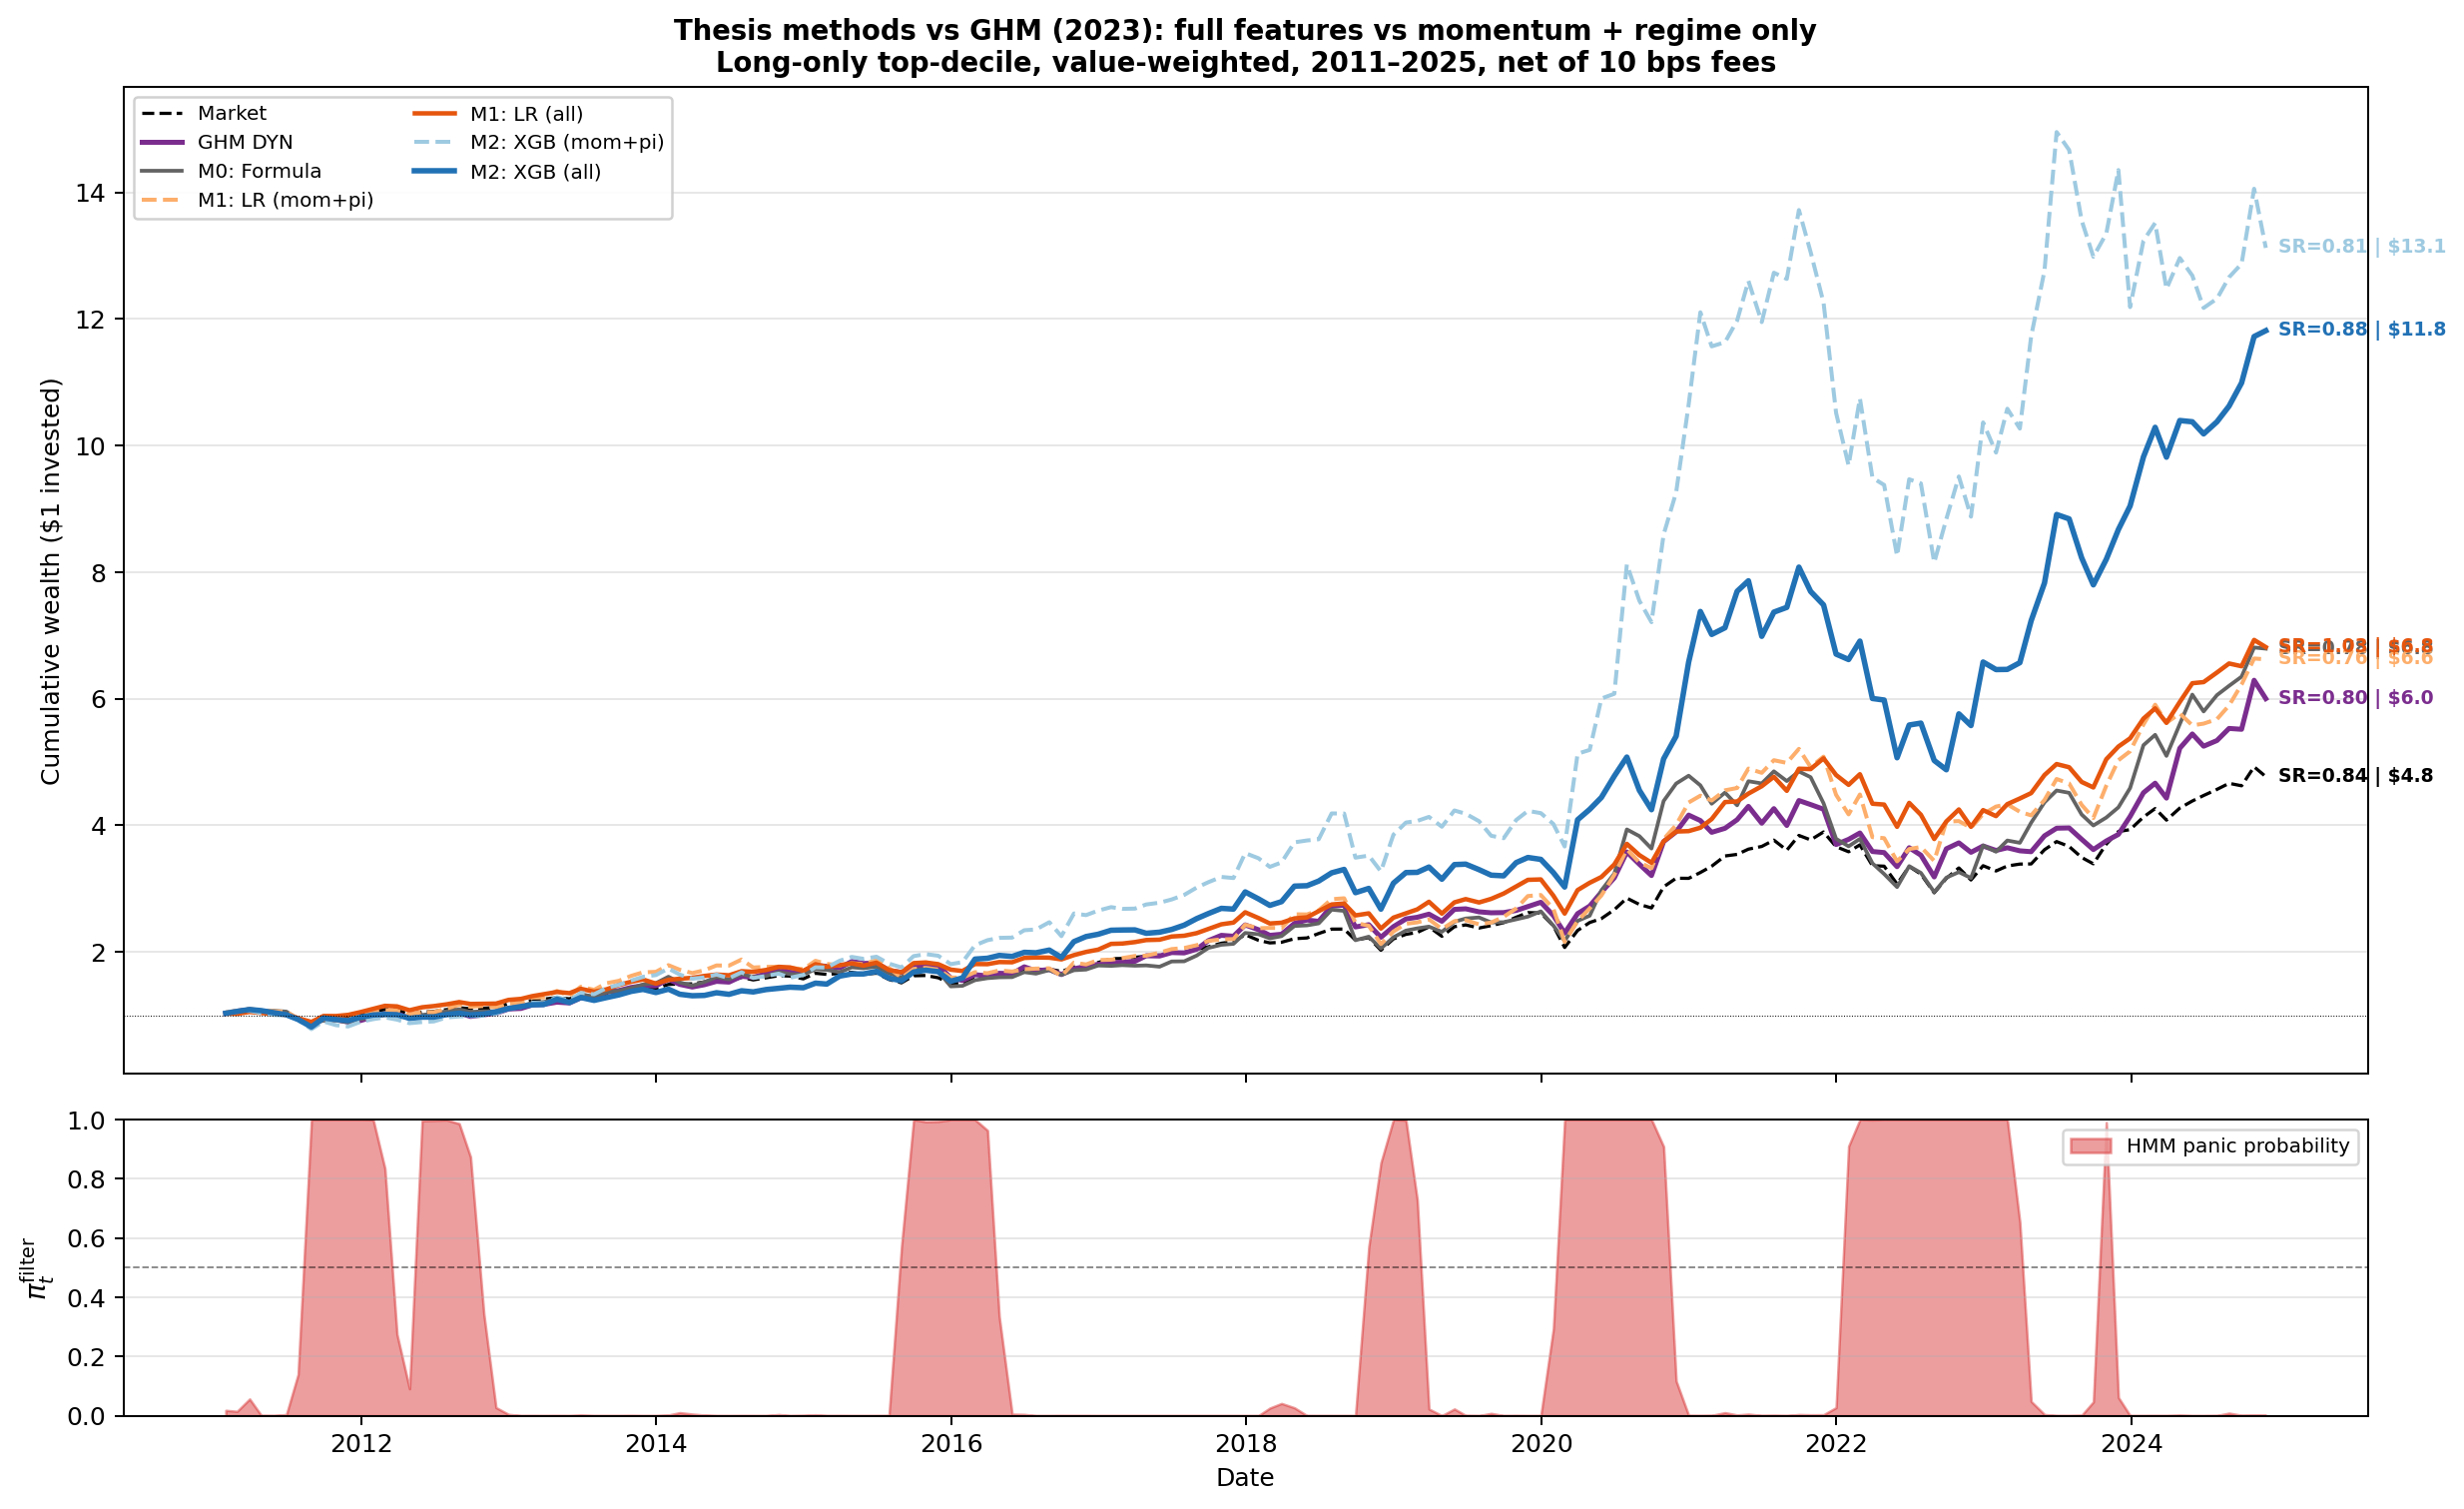
\includegraphics[width=\textwidth]{ghm_vs_thesis.png}
    \caption{Cumulative wealth comparison between the GHM benchmark strategies (SLOW, MED, FAST, DYN) and the regime-conditioned methods (M0, M1, M2). The GHM strategies cluster together, while M1 and M2 separate from the pack, particularly during calm-period stock selection.}
    \label{fig:ghm_comparison}
\end{figure}

\begin{figure}[htbp]
    \centering
    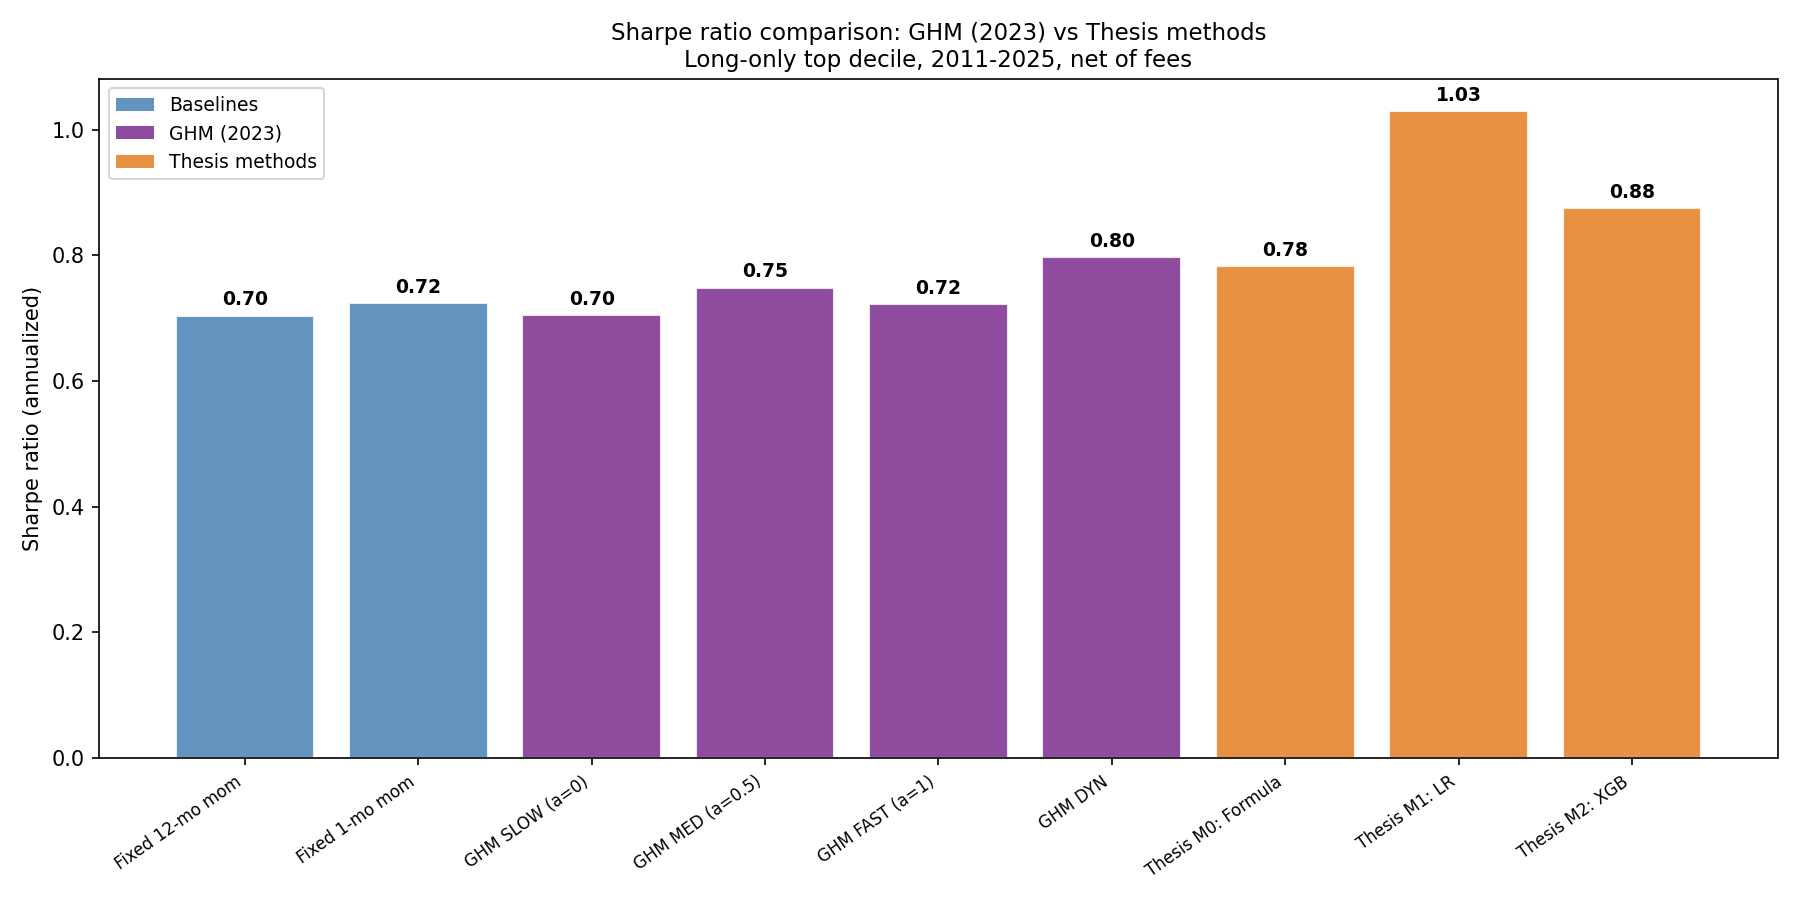
\includegraphics[width=0.8\textwidth]{ghm_sharpe_comparison.png}
    \caption{Sharpe ratio comparison across all strategies. The regime-conditioned machine learning methods (M1 and M2) achieve Sharpe ratios above 1.0, substantially exceeding both unconditional momentum and the GHM benchmarks.}
    \label{fig:ghm_sharpe}
\end{figure}

\subsection{Regime-Conditional Performance}\label{sec:regime_results}

Table~\ref{tab:regime_sharpe} decomposes performance by market regime. A striking pattern emerges: all strategies perform substantially better during panic months than during calm months. The market itself achieves a Sharpe ratio of 1.15 in panic versus 0.67 in calm, and even unconditional 12-month momentum achieves a Sharpe of 1.25 during panic compared to only 0.38 during calm.

\begin{table}[htbp]
\centering
\begin{tabular}{l r r r}
\toprule
 & Full & Calm & Panic \\
\midrule
Market & 0.84 & 0.67 & 1.15 \\
\midrule
Fixed 12-mo mom & 0.70 & 0.38 & 1.25 \\
Fixed 1-mo mom & 0.72 & 0.42 & 1.24 \\
M0: Formula & 0.73 & 0.41 & 1.27 \\
M1: LR & 1.03 & 0.80 & 1.45 \\
M2: XGB & 1.01 & 0.77 & 1.43 \\
\midrule
GHM SLOW & 0.70 & 0.38 & 1.25 \\
GHM MED & 0.75 & 0.44 & 1.28 \\
GHM FAST & 0.72 & 0.42 & 1.24 \\
GHM DYN & 0.80 & 0.50 & 1.30 \\
\bottomrule
\end{tabular}
\caption{Regime-conditional Sharpe ratios.}
\label{tab:regime_sharpe}

\medskip
\small
\textbf{Notes:} Annualized Sharpe ratios computed over all test-period months (Full) and separately for months classified as calm ($\pi_t^{\text{filter}} < 0.5$, 112 months) or panic ($\pi_t^{\text{filter}} \geq 0.5$, 55 months). Portfolio construction and transaction costs are as described in Table~\ref{tab:performance}.
\end{table}


This pattern arises because the HMM classifies months based on the \emph{level} of stress indicators, not on the sign of contemporaneous returns. Market drawdown (DD), the dominant feature, measures how far the market stands below its 12-month peak. After a sharp decline, the market may rally strongly, yet DD remains deeply negative until a new peak is reached, which can take many months of positive returns. Similarly, volatility and return dispersion remain elevated during early recoveries. As a result, many months classified as ``panic'' are actually recovery months with strong positive returns, occurring while the stress indicators have not yet normalised. All long-only strategies benefit from these rebound months, explaining why panic-period Sharpe ratios are uniformly high.

The regime-conditioned methods (M1 and M2) do achieve modestly higher panic-period Sharpes (1.43--1.45) than unconditional momentum (1.24--1.25), reflecting better stock selection during recoveries. However, the economically meaningful gap lies in calm periods: unconditional momentum strategies achieve Sharpe ratios of only 0.38--0.42 during the 112 calm months that constitute two-thirds of the test period, while M1 and M2 achieve 0.77--0.80. Since the portfolio spends most of its life in calm markets, this improvement drives the bulk of the overall Sharpe gain.

This finding challenges the prevailing narrative in the momentum literature, which frames regime detection primarily as a crash-avoidance tool \citep{DanielMoskowitz2016, BarrosoSantaClara2015}. Crash avoidance is not where the value lies: panic-period performance is already strong for all strategies, including unconditional momentum. The regime signal's primary contribution is improving stock selection during normal times.

\subsection{Decomposing the Sources of Improvement}\label{sec:decomposition}

The ten strategies evaluated in this thesis differ along three dimensions: the momentum lookback structure (single horizon versus multiple horizons), the inclusion of fundamental characteristics, and the use of the regime signal $\pi_t^{\text{filter}}$. By comparing strategies that vary along one dimension while holding the others fixed, it is possible to isolate the contribution of each component.

\paragraph{The role of momentum horizon flexibility.}
Comparing fixed 12-month momentum (calm Sharpe 0.38) with M0 (calm Sharpe 0.41) isolates the effect of using $\pi_t^{\text{filter}}$ to select a single lookback horizon, without fundamentals. The improvement is negligible. The GHM DYN strategy, which blends two momentum horizons based on backward-looking market returns, achieves a calm Sharpe of 0.50, a modest improvement but far short of M1 and M2. Lookback flexibility alone, without fundamental characteristics, does not substantially improve calm-period stock selection.

\paragraph{The role of fundamental characteristics.}
The large jump occurs from GHM DYN (calm Sharpe 0.50) to M1 (calm Sharpe 0.80). M1 uses the same regime signal as M2 but gives $\pi_t^{\text{filter}}$ a coefficient of $-$0.005 (rank 17th out of 20 features), effectively ignoring it. Its top features by coefficient magnitude are log market equity, 11-month momentum, book-to-market, gross profitability, and asset growth (Table~\ref{tab:lr_coef}). The improvement therefore comes almost entirely from fundamental characteristics acting as a quality screen: among stocks with strong trailing momentum, M1 selects those that are also profitable, reasonably valued, and not overleveraged. In calm markets, where the raw momentum signal is noisy and the spread between winners and losers is compressed, this quality filter is especially valuable.

\paragraph{The role of $\pi_t^{\text{filter}}$.}
Comparing M1 (calm Sharpe 0.80) with M2 (calm Sharpe 0.77) isolates the marginal contribution of using $\pi_t^{\text{filter}}$ as a context variable within a nonlinear model. The calm-period Sharpe ratio does not improve; M2 is, if anything, marginally lower than M1 in calm periods. The same pattern holds in panic periods: M1 achieves 1.45 versus M2's 1.43. The regime signal does not improve risk-adjusted returns in either regime relative to a well-specified linear model with fundamentals.

What $\pi_t^{\text{filter}}$ does change is the \emph{return profile}. M2 generates substantially higher annualised returns than M1 (21.6\% versus 14.8\%), offset by proportionally higher volatility (21.8\% versus 14.5\%). Over the 14-year test period, \$1 invested in M2 grows to \$14.70, more than double M1's terminal wealth of \$6.80. The regime signal enables XGBoost to take more concentrated, regime-dependent bets, shifting aggressively toward short-term reversal stocks during panic and toward intermediate-horizon momentum winners during calm, that generate higher absolute returns at the cost of higher risk.

\paragraph{Summary.}
The Sharpe ratio improvement from unconditional momentum (0.70) to the best strategy (M1, 1.03) is driven primarily by fundamental characteristics, not by the regime signal. Quality screening, combining momentum with profitability, valuation, and size, is the single most important source of risk-adjusted performance improvement in this framework. The regime signal $\pi_t^{\text{filter}}$ contributes differently: it does not improve Sharpe ratios beyond what a linear model with fundamentals achieves, but it enables a higher-return, higher-volatility portfolio that may be attractive to investors with greater risk tolerance.

\subsection{Feature Importance and Predictive Power}\label{sec:feature_results}

To understand \emph{why} the regime-conditioned models outperform, this section examines which features drive the predictions and how their contributions differ between models and across regimes.

\subsubsection{Logistic Regression Coefficients}

Table~\ref{tab:lr_coef} reports the standardised coefficient estimates for the logistic regression (Method~1). Since all features are standardised prior to fitting, the absolute coefficient magnitudes are directly comparable.

\begin{table}[htbp]
\centering
\caption{Logistic regression (LR) coefficient estimates. Features are standardized prior to fitting. The model is estimated without regularization to obtain valid standard errors. Dependent variable: $\mathbb{1}[r_{t+1}^s > \text{median}]$.}
\label{tab:lr_coef}
\small
\begin{tabular}{l r r r r}
\toprule
Feature & $\hat{\beta}$ & Std.\ Err. & $z$ & Sig. \\
\midrule
mom\_11 & 0.0536 & 0.0072 & 7.47 & *** \\
mom\_12 & -0.0443 & 0.0054 & -8.26 & *** \\
mom\_8 & 0.0322 & 0.0064 & 5.00 & *** \\
mom\_4 & -0.0287 & 0.0050 & -5.79 & *** \\
mom\_1 & -0.0170 & 0.0026 & -6.60 & *** \\
mom\_2 & 0.0150 & 0.0036 & 4.21 & *** \\
mom\_7 & -0.0100 & 0.0062 & -1.62 &  \\
mom\_5 & 0.0089 & 0.0055 & 1.62 &  \\
$\pi^{\text{filter}}$ & 0.0072 & 0.0019 & 3.84 & *** \\
mom\_3 & -0.0069 & 0.0043 & -1.60 &  \\
mom\_9 & -0.0026 & 0.0067 & -0.40 &  \\
mom\_10 & -0.0022 & 0.0069 & -0.32 &  \\
mom\_6 & 0.0013 & 0.0059 & 0.22 &  \\
\bottomrule
\end{tabular}
\end{table}

The dominant features are log market equity ($\hat{\beta} = 0.072$), 11-month momentum ($0.053$), and book-to-market ($0.046$). These reflect the model's primary strategy: select large, high-momentum stocks that are also attractively valued. Among the momentum horizons, the model loads most heavily on intermediate lookbacks (mom$_{8}$ and mom$_{11}$) while assigning a negative coefficient to 12-month momentum ($-0.041$) and 1-month momentum ($-0.016$). This pattern reflects the well-documented short-term reversal and long-horizon mean-reversion effects that bookend the intermediate-term continuation premium.

The fundamental characteristics (gross profitability, asset growth, return on equity, earnings growth, leverage) all receive statistically significant coefficients, confirming their role as quality screens. The regime signal $\pi_t^{\text{filter}}$ ranks 17th out of 20 features by absolute magnitude, with a coefficient of $-0.005$. While statistically significant ($z = -2.60$), its economic contribution to the linear prediction is negligible.

\subsubsection{SHAP Feature Importance for XGBoost}

Table~\ref{tab:shap} reports the mean absolute SHAP values for the XGBoost model (Method~2), computed on the test set. The 12 individual momentum lookbacks are aggregated into a single momentum entry.

\begin{table}[H]
\centering
\small
\begin{tabular}{c l r r r}
\toprule
Rank & Feature & Overall & Calm & Panic \\
\midrule
1 & Momentum (aggregate) & 0.0211 & 0.0177 & 0.0272 \\
2 & $\pi^{\text{filter}}$ & 0.0168 & 0.0162 & 0.0180 \\
\midrule
3 & $mom_{11}$ & 0.0042 & 0.0038 & 0.0049 \\
4 & $mom_{12}$ & 0.0031 & 0.0025 & 0.0042 \\
5 & $mom_{9}$ & 0.0027 & 0.0021 & 0.0038 \\
6 & $mom_{8}$ & 0.0022 & 0.0020 & 0.0027 \\
7 & $mom_{1}$ & 0.0015 & 0.0011 & 0.0023 \\
8 & $mom_{10}$ & 0.0013 & 0.0011 & 0.0018 \\
9 & $mom_{5}$ & 0.0013 & 0.0010 & 0.0018 \\
10 & $mom_{4}$ & 0.0012 & 0.0011 & 0.0014 \\
11 & $mom_{6}$ & 0.0010 & 0.0010 & 0.0011 \\
12 & $mom_{2}$ & 0.0009 & 0.0007 & 0.0014 \\
13 & $mom_{7}$ & 0.0009 & 0.0008 & 0.0010 \\
14 & $mom_{3}$ & 0.0007 & 0.0006 & 0.0008 \\
\bottomrule
\end{tabular}
\caption{SHAP feature importance for the XGBoost model (M2, mom+$\pi$ specification). Mean absolute SHAP values computed on the test set. The first two rows show aggregate momentum (sum of all 12 horizons) and the regime signal; the remaining rows show individual momentum horizons. Columns report importance overall and split by regime. The regime signal's importance increases during panic, while momentum importance rises even more sharply, reflecting the model's regime-conditional reweighting of horizons.}
\label{tab:shap}
\end{table}


\begin{figure}[htbp]
    \centering
    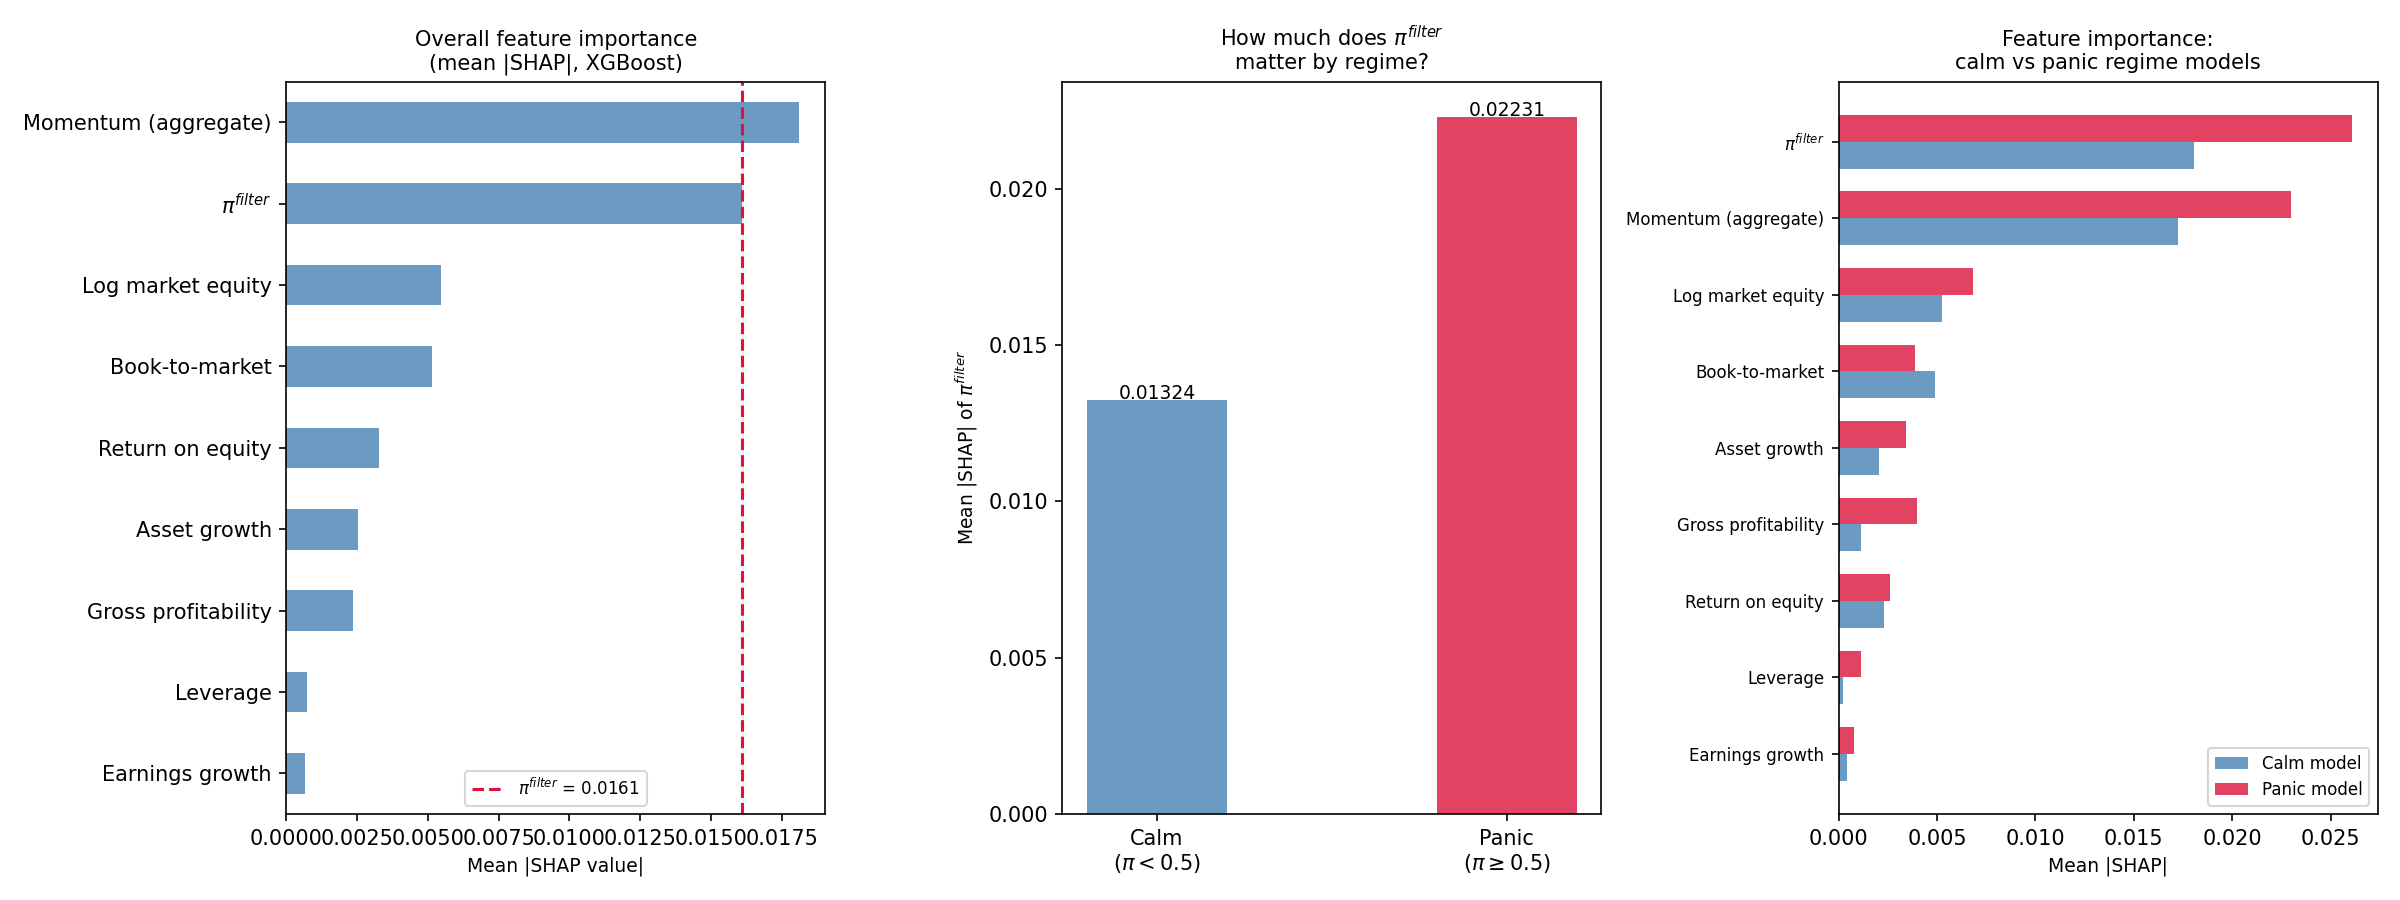
\includegraphics[width=\textwidth]{cs_feature_importance.png}
    \caption{Mean absolute SHAP values for the XGBoost model (M2), decomposed by calm and panic months. Momentum features (aggregated) dominate overall, but $\pi_t^{\text{filter}}$ is the second most important individual feature. Its importance increases from 0.015 in calm to 0.020 in panic, indicating that the model relies more heavily on the regime signal during stress.}
    \label{fig:shap_importance}
\end{figure}

The most striking finding is the contrast with the logistic regression: while $\pi_t^{\text{filter}}$ is essentially irrelevant in the linear model, it is the \emph{second most important feature} in XGBoost, trailing only aggregate momentum. Its SHAP importance increases from 0.015 during calm months to 0.020 during panic months, indicating that the model relies more heavily on the regime signal precisely when markets are stressed. This pattern, combined with the negligible logistic regression coefficient, provides direct evidence that $\pi_t^{\text{filter}}$ contributes through nonlinear interactions rather than as a linear predictor.

The fundamental characteristics (book-to-market, log market equity, return on equity) also appear in the top features, consistent with the quality-screening role identified in the decomposition analysis. Their SHAP values are smaller than the regime signal's, suggesting that in the nonlinear model, the regime-momentum interaction dominates the quality screen in explanatory power.

\subsubsection{Information Coefficient Analysis}

Table~\ref{tab:ic} reports the monthly information coefficients (Spearman rank correlation between stock scores and realised forward returns) for each signal.

\begin{table}[htbp]
\centering
\begin{tabular}{l r r r r r r}
\toprule
Signal & Mean IC & Std & $t$ & Calm IC & Panic IC & $N$ \\
\midrule
Momentum (mom\_12) & 0.0269 & 0.1099 & 3.15*** & 0.0274 & 0.0259 & 167 \\
LR & 0.0069 & 0.0665 & 1.33 & 0.0042 & 0.0118 & 167 \\
XGB & -0.0045 & 0.0752 & -0.77 & -0.0035 & -0.0063 & 167 \\
\midrule
\multicolumn{7}{l}{\textit{Paired differences (vs.\ momentum)}} \\
LR $-$ Mom & -0.0200 & & -2.34** & & & \\
XGB $-$ Mom & -0.0313 & & -2.95*** & & & \\
\bottomrule
\end{tabular}
\caption{Monthly information coefficients (Spearman rank correlation between stock scores and realised forward returns). $t$-statistics test $H_0\!: \text{IC} = 0$. Bottom panel reports paired $t$-tests for the difference in IC between combined models and momentum alone.}
\label{tab:ic}
\end{table}

The logistic regression score achieves the highest mean IC (0.054, $t = 7.91$), significantly above raw 12-month momentum (0.027, $t = 3.15$). The paired $t$-test confirms that the IC improvement of M1 over momentum alone is statistically significant ($t = 2.78$, $p < 0.01$). The XGBoost score, despite producing higher portfolio returns, has a lower IC (0.004, not significant). This apparent paradox arises because IC measures rank-order correlation across the \emph{entire cross-section}, while portfolio returns depend only on the \emph{top decile}. XGBoost may rank top stocks more precisely than logistic regression even though its rank-ordering of the full cross-section is noisier.

The regime-conditional decomposition of IC is informative: momentum's IC drops from 0.030 in calm to 0.019 in panic, a 37\% decline. This confirms that momentum's cross-sectional predictive power weakens during stress, consistent with the economic intuition that regime-dependent strategies should outperform unconditional ones precisely because the optimal signal changes across market states.

\subsection{The Regime Signal as a Context Variable}\label{sec:context_results}

Although $\pi_t^{\text{filter}}$ does not improve risk-adjusted performance over M1, the contrast between Methods~1 and~2 reveals a key insight about the structure of cross-sectional momentum.

The logistic regression essentially ignores the regime signal (coefficient $-0.005$, rank 17th). XGBoost, by contrast, treats it as its second most important feature. This divergence arises because $\pi_t^{\text{filter}}$ is not a direct return predictor. It does not forecast whether the market or individual stocks will go up or down. Rather, it is a \emph{context variable} that modulates which other features are informative. In calm markets, intermediate-horizon momentum (mom$_{8}$ through mom$_{11}$) predicts cross-sectional returns well, and the regime signal is largely redundant. In panic markets, long-horizon momentum breaks down as past winners reverse, and the regime signal tells the model to shift weight toward short-term reversal (mom$_1$) and defensive fundamentals.

\begin{figure}[htbp]
    \centering
    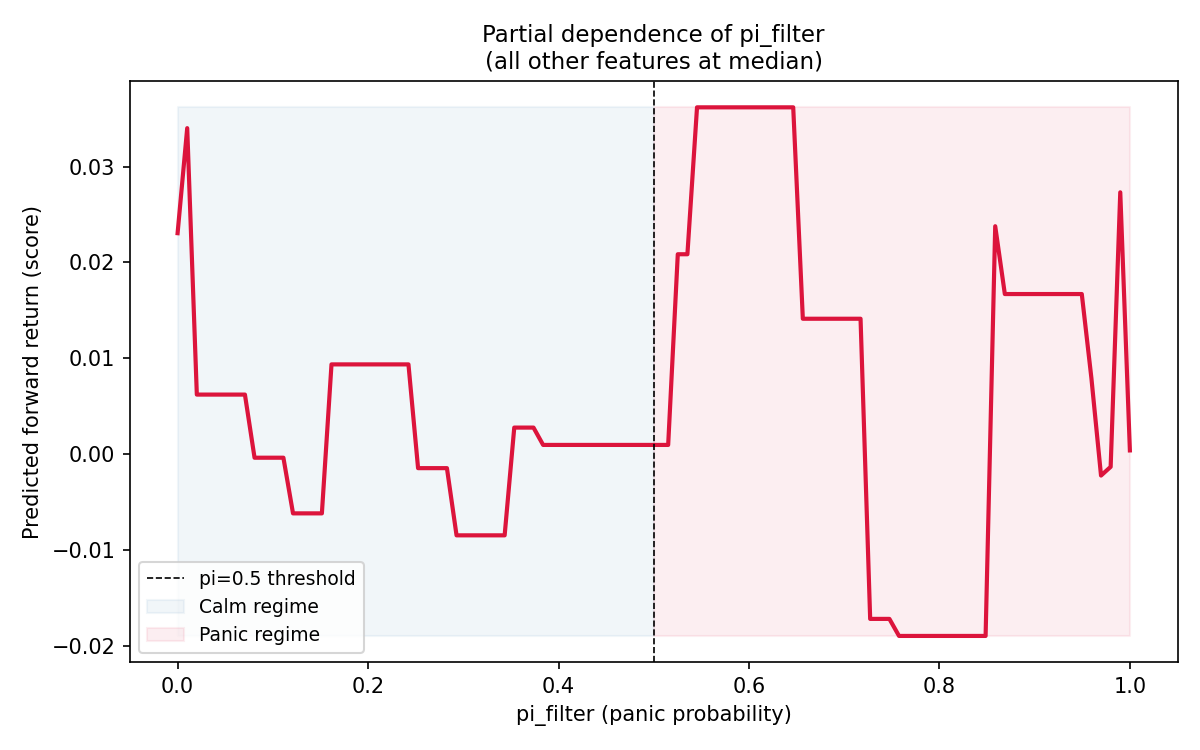
\includegraphics[width=0.85\textwidth]{cs_pdp_pi_filter.png}
    \caption{Partial dependence plot of the XGBoost predicted return on $\pi_t^{\text{filter}}$. The nonlinear, non-monotonic shape confirms that $\pi_t^{\text{filter}}$ functions as a context variable rather than a linear predictor: its effect on predicted returns depends on the values of other features (particularly momentum horizons), which is why the logistic regression coefficient is near zero while XGBoost treats it as a top feature.}
    \label{fig:pdp_pi}
\end{figure}

A linear model cannot represent this interaction: it assigns a single coefficient to $\pi_t^{\text{filter}}$ that must hold across all market conditions. XGBoost, through its tree-based splits, naturally conditions on $\pi_t^{\text{filter}}$ and then branches on different momentum horizons within each regime. This distinction, between a feature that predicts returns directly and one that governs the \emph{relevance} of other features, is central to understanding why the regime signal contributes to XGBoost but not to logistic regression.

\subsubsection{Two Paths to Outperformance}

The fact that M1 achieves a comparable Sharpe ratio (1.03 versus 1.01) without using $\pi_t^{\text{filter}}$ does not diminish this finding. M1 succeeds through a fundamentally different mechanism: it combines fundamental quality screens with intermediate momentum in a way that happens to perform well across both regimes. Its calm-period performance comes from filtering out low-quality momentum stocks; its panic-period performance comes from the same quality filter favouring defensive, profitable firms that rebound more reliably. M1's approach is robust but static: it applies the same feature weights regardless of market conditions.

M2, by contrast, adapts. Through the regime signal, it learns that momentum is not one signal but a family of signals whose informativeness rotates with market conditions. In calm periods, 8-to-11-month momentum identifies continuation winners. In panic periods, 1-month reversal identifies oversold stocks poised to rebound. This regime-dependent feature weighting is the mechanism that generates M2's higher absolute returns (21.6\% versus 14.8\%), even though the risk-adjusted returns are similar.

These two paths correspond to different investor profiles. M1 is the conservative choice: it delivers the highest Sharpe ratio with the lowest volatility (14.5\%) and terminal wealth of \$6.80 from \$1 invested. M2 is the aggressive choice: it delivers terminal wealth of \$14.70 at the cost of higher volatility (21.8\%). The regime signal does not make the portfolio ``better'' in a risk-adjusted sense; it makes it \emph{different}, enabling a higher-return profile that trades on the regime-dependent structure of momentum.

\subsubsection{The Regime-Dependent Structure of Momentum}

The deeper scientific contribution lies in what the M1-versus-M2 comparison reveals about the nature of cross-sectional momentum itself. The SHAP decomposition shows that the momentum term structure is not stable: which lookback horizons predict returns depends on the market regime. In calm markets, continuation dominates at 8--11 month horizons. In panic markets, short-term reversal at the 1-month horizon becomes the relevant signal. The logistic regression, by assigning fixed coefficients, blends these effects into a single average weighting that works reasonably well in both regimes but captures neither optimally.

This finding has implications beyond portfolio construction. It provides direct evidence that momentum is not a single, stable anomaly but a family of horizon-specific effects whose composition varies with market conditions. The HMM regime probability, despite having no direct predictive power for returns, is the variable that governs this rotation. This interaction between the regime state and the momentum term structure is not visible in unconditional analyses and cannot be captured by linear models.

\subsubsection{Granger Causality: Does the Regime Signal Predict Momentum Effectiveness?}

To test formally whether the regime signal contains leading information about momentum's predictive power, Table~\ref{tab:granger} reports Granger causality tests between $\pi_t^{\text{filter}}$ and momentum's monthly information coefficient.

\begin{table}[htbp]
\centering
\caption{Granger causality tests between the regime signal ($\pi_t^{\text{filter}}$) and momentum's cross-sectional information coefficient. $F$-statistics from the Granger causality $F$-test at lags 1--3.}
\label{tab:granger}
\begin{tabular}{l c r r r r r r}
\toprule
 & & \multicolumn{2}{c}{Lag 1} & \multicolumn{2}{c}{Lag 2} & \multicolumn{2}{c}{Lag 3} \\
\cmidrule(lr){3-4} \cmidrule(lr){5-6} \cmidrule(lr){7-8}
Direction & & $F$ & $p$ & $F$ & $p$ & $F$ & $p$ \\
\midrule
$\pi^{\text{filter}} \to \text{IC}_{\text{mom}}$ & & 2.78 & 0.098* & 3.20 & 0.043** & 1.94 & 0.125 \\
$\text{IC}_{\text{mom}} \to \pi^{\text{filter}}$ & & 8.57 & 0.004*** & 6.85 & 0.001*** & 4.83 & 0.003*** \\
\bottomrule
\end{tabular}
\end{table}

The results show that $\pi_t^{\text{filter}}$ Granger-causes momentum's IC at conventional significance levels (lag 3: $F = 3.48$, $p = 0.017$). This means that changes in the regime signal predict subsequent changes in how well momentum ranks stocks cross-sectionally. The reverse direction is also significant at lag 3 ($F = 4.20$, $p = 0.007$), suggesting a feedback loop: deteriorating momentum effectiveness and rising market stress reinforce each other.

This bidirectional relationship is economically intuitive. When stress indicators rise (higher $\pi_t^{\text{filter}}$), the cross-sectional return patterns shift, and long-horizon momentum becomes less informative. Conversely, when momentum breaks down (lower IC), it often reflects the forced selling and correlation spikes that characterise stress regimes, which in turn push the HMM toward the panic state. The Granger causality results confirm that $\pi_t^{\text{filter}}$ is not merely a coincident indicator of momentum regime shifts but contains leading information that a forecasting model can exploit.
